\documentclass[runningheads,a4paper]{llncs}

\usepackage{amssymb}
\setcounter{tocdepth}{3}
\usepackage{graphicx}
\usepackage{amsmath}
\usepackage{verbatim}
\usepackage[margin=0.9in]{geometry}
\usepackage{amsfonts}
\usepackage{subfigure}
\usepackage{mathtools}
\usepackage{caption}
\usepackage{subcaption}
\usepackage{cite}
\usepackage{hyperref}
\usepackage{url}
\urlstyle{same}
\newcommand{\keywords}[1]{\par\addvspace\baselineskip
\noindent\keywordname\enspace\ignorespaces#1}

\makeatletter
\let\c@lemma=\c@theorem
\let\c@corollary=\c@theorem
\let\c@fact=\c@theorem
\makeatother

%\let\realendproof=\endproof
%\def\end proof{\hspace*{\fill}$\Box$\realendproof}
\date{October 29th, 2014}							% Activate to display a given date or no date 

\begin{document}

\title{The NP-Completeness of Some Edge Partition Problems}
\titlerunning{}

\author{Fermi Ma \and Ariel Schvartzman \and Erik Waingarten}
%
\authorrunning{Fermi Ma \and Ariel Schvartzman \and Erik Waingarten}
% (feature abused for this document to repeat the title also on left hand pages)

% the affiliations are given next; don't give your e-mail address
% unless you accept that it will be published
\institute{Massachusetts Institute of Technology}

\maketitle

The reduction that shows that Sudoku is NP-hard follows the following pattern:\\
3SAT $\rightarrow$ EP$_n$ $\rightarrow$ Triangle Partition $\rightarrow$ Latin Squares $\rightarrow$ Sudoku. \\
Here I focus on the first reduction, from 3SAT to EP$_n$. Then second case is a trivial modification. All reductions will be parsimonious, which makes \# P-completeness follow.

\section{The Problem}

The problem EP$_n$ is the following: 
\begin{itemize}
\item Input: graph $G = (V, E)$
\item Question: is there a partition of the edges such that each partition induces a subgraph which is isomorphic to $K_n$?
\end{itemize}

\subsection{Examples}

\begin{enumerate}
\item $G = K_n$. We can trivially parititon the edge set into one partition.
\item $G = (V, E)$, where the degree of each vertex is less than $n-1$. The answer is therefore no.
\item any other non-trivial examples ...?
\end{enumerate}

\subsection{Proof Overview}

In order to show that EP$_n$ is NP-hard, we will reduce from 3SAT. We will introduce a certain type of graph that can be partitioned in exactly 2 ways. These graphs will represent the ``objects" in a 3-cnf formula: the variables, and each literal in the formula. 

We will connect the graphs by ``associating" vertices and edges in two graphs. By associating, I mean making two vertices from two different graphs be the ``same" vertex. This connects the two graphs by making some edges be part of both graphs. The effect will be that the edge partition on one graph will induce a certain edge partition on graph the other graph. 

By making the associations correctly, we will ensure that for each clause, exactly one of the three literals in the clause has a certain partition, and if a literal graph has a certain partition, then the variable graph will have a certain partition. This will finish the reduction. 

A simple visualization of an association of edges might be the following. Suppose we have two integer lattices, $A = \mathbb{Z^2}$ and $B = \mathbb{Z^2}$. We can associate the edges of the unit square together so that the edges: 
\[ \begin{array}{c} (0,0);(1,0) \\
			     (1, 0); (1, 1) \\
			     (1, 1); (0, 1) \\
			     (0, 1); (0,0) \end{array} \]
  is the same edge in graph. Visually, this means taking the two graphs $A$ and $B$, stacking them on top of each other, and then ``glueing" the unit square together in both graphs. 

\subsection{$H_{n,p}$}

We will define a graph $H_{n,p} = (V_{n,p}, E_{n,p})$ which will act as the main gadget for the reduction from 3SAT to EP$_{n}$. Remember, the property that we want is that the graph has exactly two ways to be partitioned into edges. One partition will be the assignment of True, and the other partition will be the assignment of False. 

We will define the general graph for any $n$, but since we only need the case when $n=3$. We will let 
\[ V_{n,p} = \{ x = (x_1, x_2, ..., x_n) \in \mathbb{Z}_p^n | \sum x_i = 0 \} \]
Here we are taking vertices to be points of $\mathbb{Z}_p^n$, so we have $n$-long tuples of numbers from $0, ..., p-1$. An easy computation shows
\[ |V_{n,p}| = p^{n-1} \]
Since we can pick any $n-1$ of the coordinates, and then pick the last coordinate so that $\sum x_i = 0$ modulo $p$.

For edges, we let $(x,y)$ be an edge, if $x$ and $y$ differ only at two indices, $i,j$ and the difference between these indices is $1$. 

Note that $p$ will be an additional parameter in this graph. We will use it in two ways. The first reason is that it dictates how large the graph is, this will allow us to associate edges without risking two graphs being too close to each other and making the association of edges induce some other unwated assocations. Also, it will allow us to make the graph tripartite, which will become important in the reduction from Triangle Partition to Latin Squares.

We will go through some lemmas in order to gain an intuition as to how the structure looks and to gain some comfort in working with the graph. 

\begin{lemma}
\label{lem:translation}
Suppose $x \in V_{n,p}$, then $(v_1, v_2) \in E_{n,p}$ if and only if $(v_1+x, v_2+x) \in E_{n,p}$.
\end{lemma}

\begin{proof}
The proof is almost obvious. Suppose $v_1$ and $v_2$ differ in two incides $i,j$ where $v_1(i) = v_2(i) + 1$ and $v_1(j) = v_2(j) - 1$ and everywhere else $v_1(k) = v_2(k)$. This happens if and only if $v_1(i) + x(i) = v_2(i) + x(i) + 1$ and $v_1(j) + x(j) = v_2(j) + x(j) - 1$, and $v_1(k) + x(k) = v_2(k) + x(k)$. 
\end{proof}

Lemma~\ref{lem:translation} gives us a large amount of symmetry in the graph. In particular, it tells us that each vertex looks the same. This is because we can analyze each vertex $x$ by analyzing any translation of $x$; in particular, we can analyze the vertex at the origin. 

\begin{lemma}
\label{lem:flip}
$(v_1, v_2) \in E_{n,p}$ if and only if $(-v_1, -v_2) \in E_{n,p}$
\end{lemma}

\begin{proof}
The same argument holds as above. We can multiply every equation by $-1$ and still satisfy the equations by switching $i$ and $j$.
\end{proof}

\begin{lemma}
\label{lem:perm}
Let $\pi \in S_n$ be a permutation of $n$ elements. $(v_1, v_2) \in E_{n,p}$ if and only if $(\pi(v_1), \pi(v_2)) \in E_{n,p}$, where $\pi(v)$ acts by permuting the indices according to the permutation. 
\end{lemma}

\begin{proof}
This is also a very simple argument, since the permutation acts on both vertices equally, the two indices $i$ and $j$ are sent to some other $i'$ and $j'$ according to the permutation.
\end{proof}

Now we know that we can translate vertices and flip signs of everything, permute the indices, and still maintain isomorphic graphs. These symmetries reduce the arguments by a large amount. In particular, we will use Lemma~\ref{lem:translation}, Lemma~\ref{lem:flip}, and Lemma~\ref{lem:perm} to prove statements about the graphs by only analyzing one case. It means that when making statements about an edge in the graph, we might as well assume that edge connects the vertex at $0 = (0,0,\dots, 0)$ and a neighbor of $0$ with the first coordinate being $1$. 

\begin{lemma}
The degree of each vertex is $2\dbinom{n}{2}$.
\end{lemma}

\begin{proof}
Note that we can analyze each vertex by just analyzing the degree of $0 = (0, ..., 0)$ since we can translate by any element. We can count the neighbors of 0 by counting the indices of the coordinates where the values differ. For each $i < j \in \{ 1, ..., n\}$, we can pick either make $i = 1$ and $j = -1$, or $i = -1$ and $j = 1$. These are all neighbors of $0$. Since there are $\dbinom{n}{2}$ ways to pick ordered indices from $\{1, ..., n\}$ and each option has two possible assignments, there are $2\dbinom{n}{2}$ neighbors.
\end{proof}

\begin{lemma}
\label{lem:largestcomplete}
The largest complete subgraph is $K_n$, and any $K_3$ is contained in a unique $K_n$.
\end{lemma}

\begin{proof}
First, we show that $K_n$ is a subgraph. We can take 
\[ \begin{array}{ccccc} (0, &0, &0, &\dots, &0) \\
			     (1, &-1, &0, &\dots, &0) \\
			     (1, &0, &-1, &\dots, &0) \\
				&&\vdots \\
			     (1, &0, &0, &\dots, &-1) \end{array} \]
This subgraph is isomorphic to $K_n$. Suppose we had $K_{n+1}$ as a subgraph, we could translate the graph, flip the graph, and permute the indices of the graph in order to get the first $n$ points of the graph to be the ones listed above. Its clear to see that any other vertex will not be connected to all of them.

Now suppose we had $K_3$, with $x_1, x_2,$ and $x_3$. Then we can translate all the elements by $-x_1$, so that we are looking at $0, x, y$. Without loss of generality, we can say that the first coordinate of $x$ is 1 and there is a $-1$ at index $j$. 

So now we can look at the values of $y$ at indices $1$ and $j$. I claim that either $y(1) = 1$, or $y(j) = -1$. Suppose $y(1) \neq 1$ and $y(j) \neq -1$, then $y(1) = y(j) = 0$, since it has an edge to $0$, but then there is no edge to $y$ since there are $4$ values for which $x$ and $y$ differ. 

Once we have this, if $y(1) = 1$, $0,x, y$ sits inside the $K_n$ described above. If $y(j) = -1$, then up to a permutation of indices, $0, -x, -y$ sits inside the $K_n$ described above.
\end{proof}

We will refer to the $K_n$ has $1$'s in the same coordinate as $K$ and the $K_n$ that has $-1$ in the same coordinate as $-K$. 

\begin{lemma}
Each vertex is contained in $2n$ subgraphs isomorphic to $K_n$. 
\end{lemma}

\begin{proof}
We know that a cyclic permutation of the elements will produce disjoint $K_n$ which look like the above $K$ or like the negative of the above,  $-K$ in the Lemma~\ref{largestcomplete}. There are $n$ cyclic permutations, so there are $2n$ disjoint $K_n$ containing $0$. By Lemma~\ref{lem:translation}, we can extend this result to each vertex.
\end{proof}

\begin{lemma}
Each edge occurs in just two $K_n$.
\end{lemma}

\begin{proof}
We just need to check the edges incident on 0. Suppose the edge connects $0$ and $x$, then if the edge is a part of three distinct $K_n$, then there must be three vertices $a, b, c$ such that each one is one of the distinct $K_n$. We know that two of the three vertices $a, b$, and $c$ must be equal since either the $i$ index is the same, or the $j$ index must the same to $x$ (this follows by the same argument as in Lemma~\ref{lem:largestcomplete}). Therefore, some $K_3$ is inside two of the $K_n$, and so by the Lemma~\ref{lem:largestcomplete}, they are the same $K_n$.
\end{proof}

\begin{lemma}
Each distinct $K_n$ are either edge-disjoint, or have just one edge in common.
\end{lemma}

\begin{proof}
If there were two edges in common, then they both contain the same $K_3$, which generates the same unique $K_n$. 
\end{proof}

\begin{lemma}
\label{lem:distinctpart}
There are just two distinct edge partitions of $H_{n,p}$ into $K_n$'s.
\end{lemma}

\begin{proof}
Suppose $\Pi$ is an edge partition, and we have some edge $e$ being part of some $K_n$. Then $K_n$ looks like $K$ or $-K$ after some translation to the origin. If $K_n$ looks like $K$, then every other partition containing an edge incident on $0$ will be part of a $K_n$ that looks like $K$. Note that if it looked like $-K$, then it would share an edge. 

Since the graph is connected, there is a path from each edge to another edge. In each edge, they are incident on the same vertex. After translating each vertex to 0, its clear that all edges on the path will be part of some $K_n$ that looks like $K$, and since translation preserves signs, all edges on the path between two edges is part of a complete graph that looks like $K$. This means that every edge in the partition belongs to some $K_n$ that looks like $K$.

The same argument holds for $-K$. This means that the partition of a single $K_n$ determines the partition of the entire graph. Either it is determined by the the edge from $0$ to $(1, -1, 0, \dots, 0)$ being part of $K$, or $-K$. This means there are two ways to partition the graph.  
\end{proof}

Now we will let $T$-partitions of $H_{n,p}$ correspond to the edge $e$ connecting $0$ and $x = (1, -1, 0, \dots, 0)$ being part of $K$ and $F$-partitions of $H_{n,p}$ correspond to the edge $e$ being part of $-K$. Note that by Lemma~\ref{lem:distinctpart}, these are two mutually exclusive partitions of $H_{n,p}$.

\subsection{Special case when $n=3$}

For our case, we care about $n=3$. We can think of the graph as looking like perfect triangle packing of smaller equilateral triangles, with some additional edges on the sides.

\begin{figure}[h]
\label{fig:H3at0}
\centering
\includegraphics[width=0.5\linewidth]{h3at0.pdf}
\caption{$H_{3,p}$ near vertex $(0,0,0)$}
\end{figure}

We can look at what the graph looks like near the 0 vertex (see Figure~\ref{fig:H3at0}).
If we rotate to see the plane $x + y + z = 0$ on the paper, then we will get the graph with a equilateral triangle tiling of the plane. Where the shapes will look like repeating values of Figure~\ref{fig:triangletiling}.

\begin{figure}[h]
\label{fig:triangletiling}
\centering
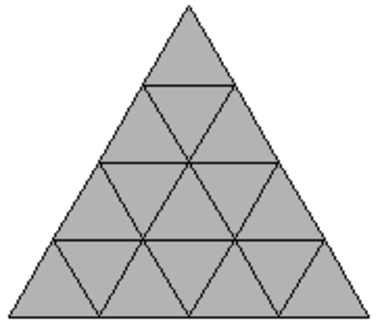
\includegraphics[width=0.2\linewidth]{EdgePartitionPic1.pdf}
\caption{Equilateral triangular tiling of the plane}
\end{figure}

Note that all side lengths are even, so when we compose these, the side lengths will be even. We can therefore, add edges on the sides by 2's and edges connecting the three points, and this will have exactly two ways of being partitioned. 

The reduction will take a big enough graph such that we can associate various triangles with each other. So we won't worry much about how we partition the ``ends" of the graph. A possible example is the following

The partition adding of the edges is shown in Figure~\ref{fig:edgecases} and their partitions are shown next to it. A green circle means that the triangle with green as the interior is a partition. The green circle not contained in any triangle signifies that the outer edges form a triangle. Note that we can increase the size of the graph by doubling the side lengths, which will mean that the exposed sides will have additional edges connecting the three new ends. 
\begin{figure}[b]
\label{fig:edgecases}
\centering
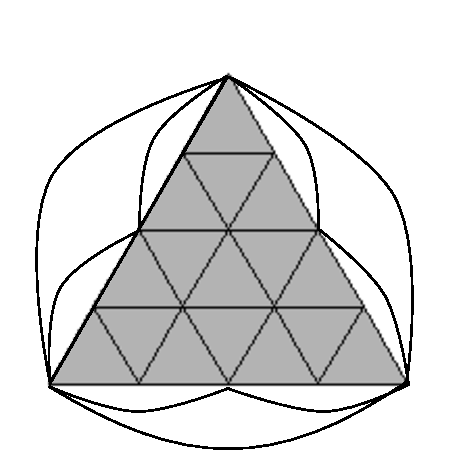
\includegraphics[width=0.2\linewidth]{triangleGraph.pdf} \qquad
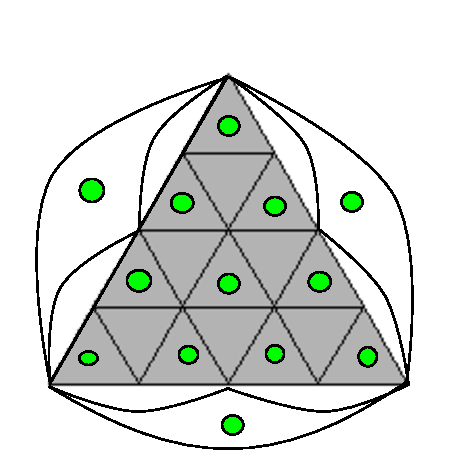
\includegraphics[width=0.2\linewidth]{triangleGraphT.pdf} \qquad
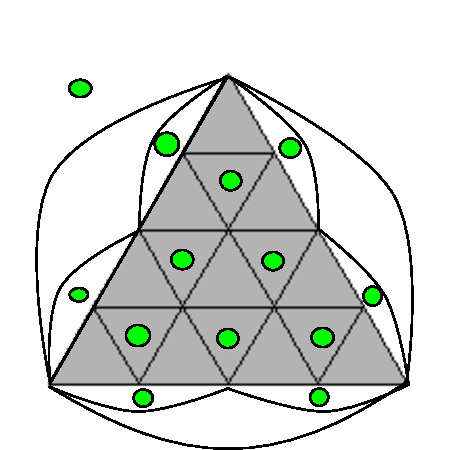
\includegraphics[width=0.2\linewidth]{triangleGraphF.pdf}
\caption{Fixing the ends of the graph and their corresponding partition}
\end{figure}

In general, $H_{n,p}$ does something similar, but with higher value cliques. The $p$ represents how tall the triangle is. 

\section{NP-hardness}

\subsection{Patches}

Now that we understand the graph, we can reduce from 3 SAT. We will have copies of the above triangle graph that are large enough to contain many \emph{patches}. By a patch, we mean the packing of the four triangles. An $F$-patch is an upward facing patch, and a $T$-patch is a downward facing path (see Figure~\ref{fig:patches}).

\begin{figure}[h]
\label{fig:patches}
\centering
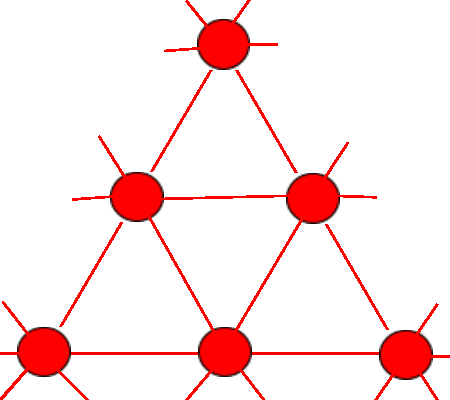
\includegraphics[width=0.2\linewidth]{Tpatch.pdf} \qquad
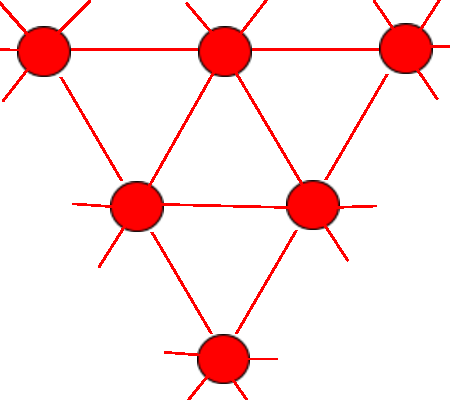
\includegraphics[width=0.2\linewidth]{Fpatch.pdf}
\caption{$F$-patch and $T$-patch}
\end{figure}

We will call a partition of a graph a \emph{$T$-partitioned} if every $T$-patch is partitioned into 3 triangles. We will call a partition of a graph an \emph{$F$-partitioned} if every $F$-patch is partitioned into $3$ triangles. Therefore, an $F$-partition will look like the middle partition in Figure~\ref{fig:edgecases}, and a $T$-partition will look like the left partition in Figure~\ref{fig:edgecases}.

\begin{definition}
In two $T$-patches or two $F$-patches, $P_1$ and $P_2$, vertices $v_1 \in P_1$ and $v_2 \in P_2$ correspond if $v_1$ and $v_2$ are in the same relative position. In a $T$-patch $P_1$ and an $F$-patch $P_2$, $v_1$ and $v_2$ correspond if they are in the same relative position after a rotation of 180 degrees.
\end{definition}

This definition corresponds the obvious elements. Two $F$-patches will have the topmost elements corresponding, the leftmost elements corresponding, and the rightmost elements corresponding. 

\subsection{Associations}

We will define an association of the graph that will have certain usefull properties. We will later use these associations to transfer information between the gadgets in the reduction. The definitions will be slightly technical. The main idea is fairly straight forward. The main idea is that we will take two graphs, and we will associate two vertices from each graph as one vertex. 

\begin{definition}
Let $G_1 = (V_1, E_1)$ and $G_2 = (V_2, E_2)$. Suppose $A \subset V_1 \times V_2$ such that
if $(v_1, v_2) \in A$, then if $(v_1, x) \in A$, $x = v_2$ and if $(x, v_2) \in A$, then $x = v_1$. Then $A$ is a valid association set of $G_1$ and $G_2$. 
\end{definition}

We require this definition so that we are associating one vertex from each graph. For our purposes, we don't need to make any more complicated associations.

\begin{definition}
Suppose $G_1 = (V_1, E_1)$, $G_2 = (V_2, E_2)$ and $A$ be a valid association set of $G_1$ and $G_2$, then let $\pi: V_1 \cup V_2 \rightarrow V_1 \cup V_2$ where
\[ \pi(v) = \left\{ \begin{array}{cc} v_1 & \text{if } v \in V_2 \text{ and } (v_1, v) \in A \\
							v & \text{ otherwise }
						      \end{array} \right. \]
and we let $V_1 \cup V_2 / A = \pi(V_1 \cup V_2)$.
\end{definition}

\begin{definition}
We let $G'$ be the association of $G_1$ and $G_2$ according to a valid association set $A$ with vertex set $V'$ and edge set $E'$ where:
\begin{itemize}
\item $V' = (V_1 \cup V_2) / A$
\item $(a,b) \in E'$ if $\pi^{-1}(a) \times \pi^{-1}(b) \cap (E_1 \cup E_2) \neq \emptyset$
\end{itemize}
We write $G' = G_1 \cup G_2 / A$.
\end{definition}

The definition for the edge set $E'$ is a bit dense. The imporant thing to note is that an edge is included in the association if it was an edge of the graphs associated. This ensures that the graph does not introduce multiple edges. The association does exactly what we want it to do: it takes two graphs $G_1$ and $G_2$ and tuples of vertices with one from each graph, and it ``glues" the vertices according to the tuples. 

Take the following simple example. Let $G_1 = (V_1, E_1)$ be a chain of $n$ elements. So $V_1 = [n]$ and $(i, i+1) \in E_1$. Likewise, we will let $G_2$ be a chain of $m$ elements. So $V_2 = [m']$ and $(i', (i+1)')\in E_2$ (note that we used primes so that the sets are disjoint). Then if we let $A = \{ (0, 0') \}$, we will have $G' = G_1 \cup G_2 / A$ with a chain of length $n+m$. If we let $A = \{ (n-1, m-1), (n-2, m-2) \}$, we will have $G' = G_1 \cup G_2 / A$ be two chains which come together for one edge, and then seperate again for one edge each (see Figure~\ref{fig:assocationexample}).

\begin{figure}[ht]
\label{fig:associationexample}
\centering
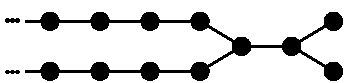
\includegraphics[width=0.5\linewidth]{associationchainexample.pdf}
\caption{Two chains assocated at one edge}
\end{figure} 

\begin{lemma}
\label{lem:varF}
Let $G_1 = H_{3, p}$ and $G_2 = H_{3, p}$ where $p$ is a large constant. Let $P_1$ be an $F$-patch in $G_1$ and $P_2$ be an $F$-patch in $G_2$. Let $A$ be the set of tuples of elements from $P_1$ and $P_2$ which correspond. Let $\Pi$ be a partition of $G_1 \cup G_2 / A$ into triangles. If $\Pi$ on $G_1$ is an $T$-partition, then $\Pi$ on $G_2 - P_2$ is a $F$-partition.
\end{lemma}

\begin{proof}
If $\Pi$ on $G_1$ is a $T$-partition, then $P_1$ will be contain only one triangle in the partition. Which means that the edges on the outside of $P_1$ will be part of triangles in the neighboring $T$-patches. So the partition of $G_2$ will be indistinguishable as if $P_2$ were a $F$-partition. And since one $F$-patch determines the partition of the whole graph, $\Pi$ on $G_2$ is $F$-partitioned.  

Figure~\ref{fig:Tpatchpartitioned} shows the $F$-patch $P_1$. The green edges corresponds to the triangle belonging to the $T$-partition of $G_1$. Also, the black edges are part of triangles of the neighboring $T$-patches on $G_1$. Therefore, to any patch in $G_2$, $P_2$ might as well have had $3$ triangles in it.
\end{proof}

\begin{figure}[t]
\label{fig:Tpatchpartitioned}
\centering
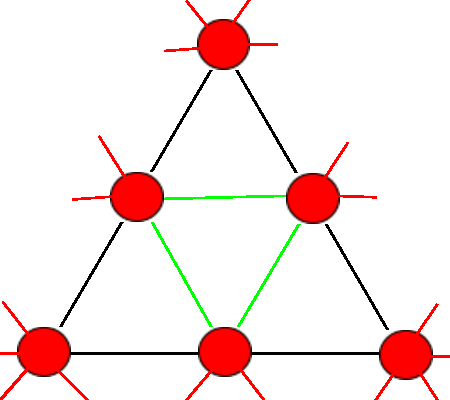
\includegraphics[width=0.2\linewidth]{TpatchPartitioned.pdf}
\caption{$G_2$ partition indistinguishable $F$-patch}
\end{figure}

Note that this proof also shows that a triangle partition after the association exists.

\begin{corollary}
\label{cor:varT}
If we associate an $F$-patch, $P_1$, of $G_1$ with an $T$-patch, $P_2$, of $G_2$, then if $\Pi$ on $G_1$ is a $T$-partition, then $\Pi$ on $G_2-P_2$ is an $T$-partition.
\end{corollary}

\begin{proof}
The same proof holds, except since we are flipping the patch, the partition of $G_2$ is inverted.
\end{proof}

\begin{lemma}
\label{lem:clause}
If we associate three graphs $G_1 = H_{3,p}$, $G_2 = H_{3,p}$, and $G_3 = H_{3,p}$ at some $F$-patch, and we remove the inner triangle of the $F$-patch, then in an edge partition of triangles, exactly one of the graphs must be a $T$-partition, and the rest must be an $F$-partition.
\end{lemma}

\begin{proof}
If we associate three $F$-patches and we remove the middle triangle, then the outer edges of the $F$-partition must be part of triangles for $T$-partitions of some graph. This means that one graph must be $T$-partitioned. The following the same arguments of Lemma~\ref{lem:varF}, the other graphs must be $F$-partitioned.
\end{proof}

\subsection{Reduction}

\begin{theorem}
EP$_3$ is NP-hard.
\end{theorem}

\begin{proof}

The reduction is from 3SAT. Let's say $\phi$ is a 3-cnf formula with $n$ variables and $c$ clauses. We will have one graph $H_{3,p}$ for each variable, and one graph $H_{3,p}$ for each literal of each clause. 

We will choose $p$ to have a large enough graph. We want there to be many $T$-patches and $F$-patches. We also want that these patches be far away from each other, so that the associations do not interfere. In particular, we want there to be at least $3c$ patches, where $c$ will be the number of clauses in the 3-cnf formula. We can require that the distance between each patch (in a graph theoretic sense) is at least 10. Therefore, if we let $p > 30c$, we will have a large enough graph. 

So now what we will have one $H_{n,p}$ for each variable, and three for each clause. We call $U_i$ the graph $H_{3,p}$ of variable $u_i$ and $C_{i,l}$ the graph $H_{3,p}$ of the $l$th literal of the $i$th clause. If the $l$th literal of clause $i$ is $u$, then we associate a $F$-patch of $C_{i,l}$ to an $T$-patch of $U_i$. If $\overline{u}$ is the $l$th literal of clause $i$, then we associate an $F$-patch to an $F$-patch of $U_i$. 

Also, we associate three $F$-patches with each other for each $C_{i, 1}, C_{i,2}$ and $C_{i,3}$. By Lemma~\ref{lem:clause}, exactly one of the three graphs $C_{i,l}$ will be a $T$-partition, and the other two will be $F$-partitions. Suppose $C_{i,l}$ is a $T$-partition, if the $l$th literal of clause $i$ is $u$, then $U_i$ will be a $T$-partition by Corollary~\ref{cor:varT}, and if the $l$th literal of clause $i$ is $\overline{u}$, then $U_i$ will be an $F$-partition by Lemma~\ref{lem:varF}.

Therefore, if the 3SAT formula has a satisfying assignment, then we make $U_i$ be a $T$-partition if $u$ is true, and an $F$-partition if $u$ is false. Then we make $C_{i,l}$ a $T$-partition if the $l$th literal is set to true and $C_{i, j}$ for $j < l$ is an $F$-partition. This will be a valid edge partition of the graph into triangles. 

If there is a valid edge partition into triangles, then exactly one of $C_{i,l}$ is a $T$-partition for each $i$, which means that at least one literal is set to true. So we let variable the $i$th variable be true if $U_i$ is a $T$-partition, and false othewise. 
\end{proof}

\bibliographystyle{plain}
\bibliography{references}

\end{document}  
